\documentclass{beamer}
\usetheme{Berlin}
% \usecolortheme{seagull}
\usecolortheme{rose}
%\setbeamertemplate{footline} % To remove the footer line in all slides uncomment this line
\setbeamertemplate{footline}[page number] % To replace the footer line in all slides with a simple slide count uncomment this line
\setbeamertemplate{navigation symbols}{} % To remove the navigation symbols from the bottom of all slides uncomment this line
\usepackage{graphicx, booktabs} 

\title{Multi-Agents and Agent Systems}
\subtitle{Flying Saucers Bakery}
\author{Md Zahidussaman, Arun Prabhu, Dharmin Bakaraniya}
\institute{H-BRS}
\date{\today}
\begin{document}

\begin{frame}
    \titlepage
\end{frame}

\begin{frame}{Overview}
    \tableofcontents
\end{frame}

\section{Baking stage}%
\label{sec:baking_stage}
\begin{frame}
    \frametitle{\huge{Baking Stage}}
    \begin{columns}[t]
        \column{.45\textwidth}
        \begin{figure}[H]
            \centering
            % \caption{Baking stage component diagram\label{fig:baking_component_diagram} }
            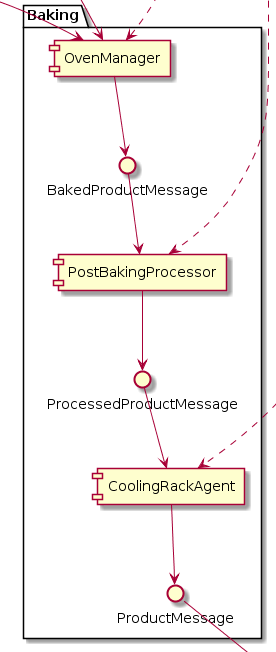
\includegraphics[width=0.6\linewidth]{baking_component_diagram.png}
        \end{figure}
        \column{.5\textwidth}
            \textbf{Agents}
            \begin{itemize}
                \item OvenManager
                \item PostBakingProcessor
                \item CoolingRackAgent
            \end{itemize}
    \end{columns}
\end{frame}
\begin{frame}
    \frametitle{\huge{OvenManager}}
    \begin{columns}[t]
        \column{.45\textwidth}
        \begin{figure}[H]
            \centering
            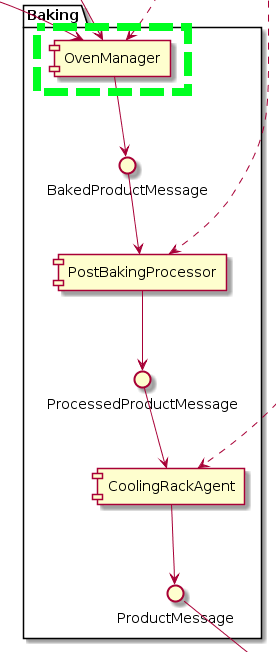
\includegraphics[width=0.6\linewidth]{baking_OvenManager.png}
        \end{figure}
        \column{.5\textwidth}
            %\textbf{OvenManager}
            \begin{itemize}
                \item Single Agent to manage all the ovens in the bakery.
                \item Receives UnbakedProductMessage
from Proofer(Dough Preparation Stage).
                \item Sends BakedProductMessage
to PostBakingProcessor(Baking Stage).
            \end{itemize}
    \end{columns}
\end{frame}
\begin{frame}
    \frametitle{\huge{PostBakingProcessor}}
    \begin{columns}[t]
        \column{.45\textwidth}
        \begin{figure}[H]
            \centering
            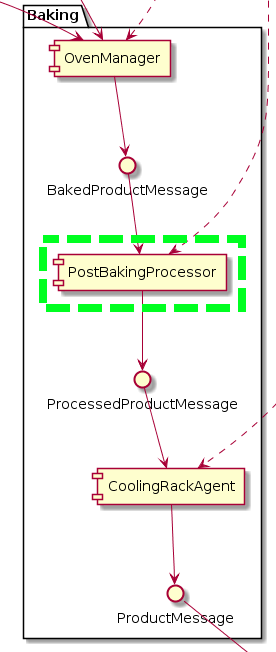
\includegraphics[width=0.6\linewidth]{baking_PostBakingProcessor.png}
        \end{figure}
        \column{.5\textwidth}
            %\textbf{PostBakingProcessor}
            \begin{itemize}
                \item Performs all the steps in the recipe of a product which occur between Baking and Cooling.
                \item Receives BakedProductMessage from OvenManager(Baking Stage).
                \item Sends the ProcessedProductMessage to CoolingRackAgent(Baking Stage).
            \end{itemize}
    \end{columns}
\end{frame}
\begin{frame}
    \frametitle{\huge{CoolingRackAgent}}
    \begin{columns}[t]
        \column{.45\textwidth}
        \begin{figure}[H]
            \centering
            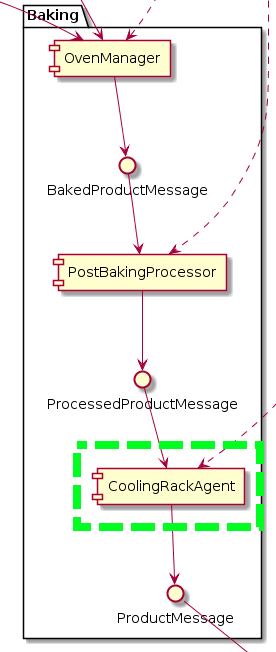
\includegraphics[width=0.6\linewidth]{baking_CoolingRackAgent.png}
        \end{figure}
        \column{.5\textwidth}
            %\textbf{CoolingRackAgent}
            \begin{itemize}
                \item Performs cooling steps of the recipe corresponding to different products. 
                \item Receives ProcessedProductMessage from PostBakingProcessor(Baking Stage).
                \item Sends
ProductMessage to PreLoadingProcessor(Packaging Stage).
            \end{itemize}
    \end{columns}
\end{frame}

\section{Packaging stage}%
\label{sec:packaging_stage}
\begin{frame}
    \frametitle{\huge{Packaging Stage}}
    \begin{columns}[t]
        \column{.45\textwidth}
        \begin{figure}[H]
            \centering
            % \caption{Baking stage component diagram\label{fig:baking_component_diagram} }
            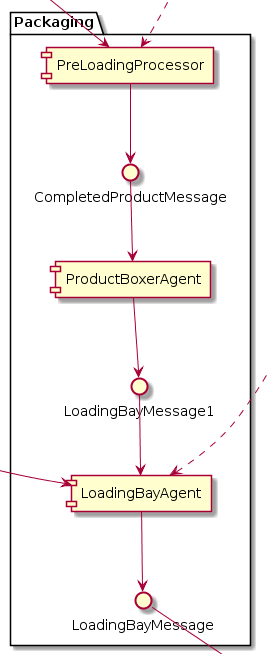
\includegraphics[width=0.55\linewidth]{packaging_component_diagram.png}
        \end{figure}
        \column{.5\textwidth}
            \textbf{Agents}
            \begin{itemize}
                \item PreLoadingProcessor
                \item ProductBoxerAgent
                \item LoadingBayAgent
            \end{itemize}
    \end{columns}
\end{frame}
\begin{frame}
    \frametitle{\huge{PreLoadingProcessor}}
    \begin{columns}[t]
        \column{.45\textwidth}
        \begin{figure}[H]
            \centering
            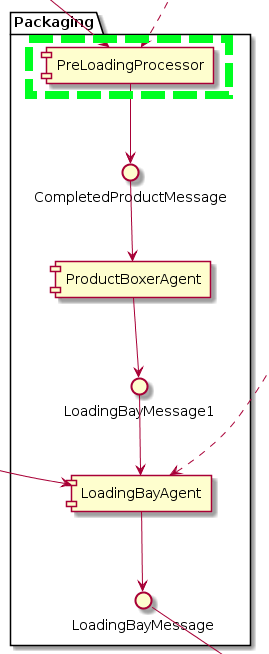
\includegraphics[width=0.55\linewidth]{pre_loading.png}
        \end{figure}
        \column{.5\textwidth}
            %\textbf{PreLoadingProcessor}
            \begin{itemize}
                \item Performs all steps in recipe of a product which lie between Cooling and Packaging.
                \item Recieves ProductMessage from CoolingRackAgent(Baking Stage).
                \item Sends CompletedProductMessage to ProductBoxerAgent(Packaging Stage).
            \end{itemize}
    \end{columns}
\end{frame}
\begin{frame}
    \frametitle{\huge{ProductBoxerAgent}}
    \begin{columns}[t]
        \column{.45\textwidth}
        \begin{figure}[H]
            \centering
            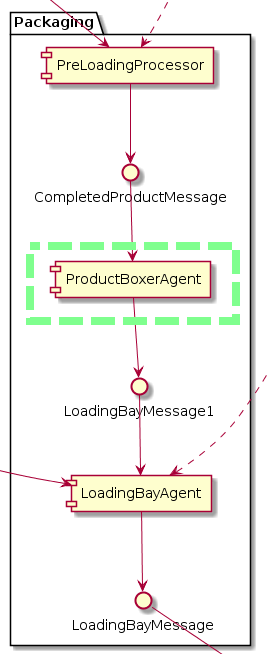
\includegraphics[width=0.55\linewidth]{productboxer.png}
        \end{figure}
        \column{.5\textwidth}
            %\textbf{ProductBoxerAgent}
            \begin{itemize}
                \item Packs the products into boxes and dispatches them.
                \item Receives CompletedProductMessage from
the PreLoadingProcessor(Packaging Stage).
                \item Sends LoadingBayMessage to the LoadingBay agent(Delivery Stage).
            \end{itemize}
    \end{columns}
\end{frame}

\section{Common agents}%
\label{sec:common_agents}
\begin{frame}
    \frametitle{\huge{Common agents}}
    \begin{columns}[t]
        \column{.45\textwidth}
        \begin{figure}[H]
            \centering
            % \caption{Baking stage component diagram\label{fig:baking_component_diagram} }
            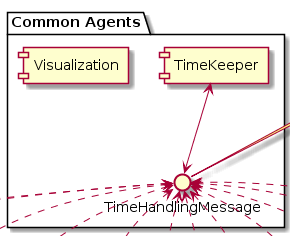
\includegraphics[width=0.75\linewidth]{common_component_diagram.png}
        \end{figure}
        \column{.5\textwidth}
            \textbf{Agents}
            \begin{itemize}
                \item TimeKeeper
                \item BaseAgent
                \item VisualisationAgent (Order board)
            \end{itemize}
    \end{columns}
\end{frame}
\begin{frame}
    \frametitle{\huge{TimeKeeper}}
    \begin{columns}[t]
        \column{.45\textwidth}
        \begin{figure}[H]
            \centering
            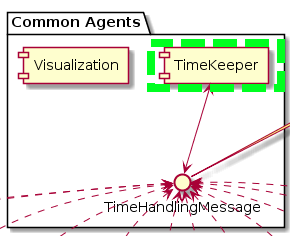
\includegraphics[width=0.75\linewidth]{common_TimeKeeper.png}
        \end{figure}
        \column{.5\textwidth}
            %\textbf{TimeKeeper}
            \begin{itemize}
                \item It is responsible for the movement of time in the entire bakery eco-system.
                \item Receives finished from the based agents of all the agents.
                \item Sends TimeStep to all the base agents of all the agents.
            \end{itemize}
    \end{columns}
\end{frame}
\begin{frame}
    \frametitle{\huge{BaseAgent}}
            \begin{itemize}
                \item BaseAgent is a parent to all agents in bakery simulation.
                \item Receives TimeStep from the TimeKeeper agent.
                \item Sends finished to the TimeKeeper agent. Sends all the messages to the visualization agents.
            \end{itemize}
\end{frame}
\begin{frame}
    \frametitle{\huge{Order Board Visualisation Agent}}
    \begin{columns}[t]
        \column{.45\textwidth}
        \begin{figure}[H]
            \centering
            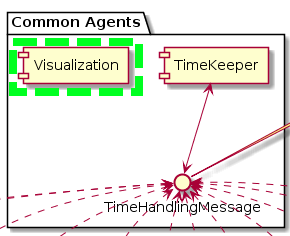
\includegraphics[width=0.75\linewidth]{common_Visualization.png}
        \end{figure}
        \column{.5\textwidth}
            %\textbf{Agents}
            \begin{itemize}
                \item Creates an instance of JavaFX application instance Visualizer during initialization and forwards all interface agent messages to the Visualizer instance.
                \item Receives the output messages of all the
interface agents(via their Base Agents).
                \item Does not send any messages apart from TimeStep finished message.
            \end{itemize}
    \end{columns}
\end{frame}

\begin{frame}
    \frametitle{\huge{Order Board Visualisation Agent}}
    \begin{figure}[H]
            \centering
            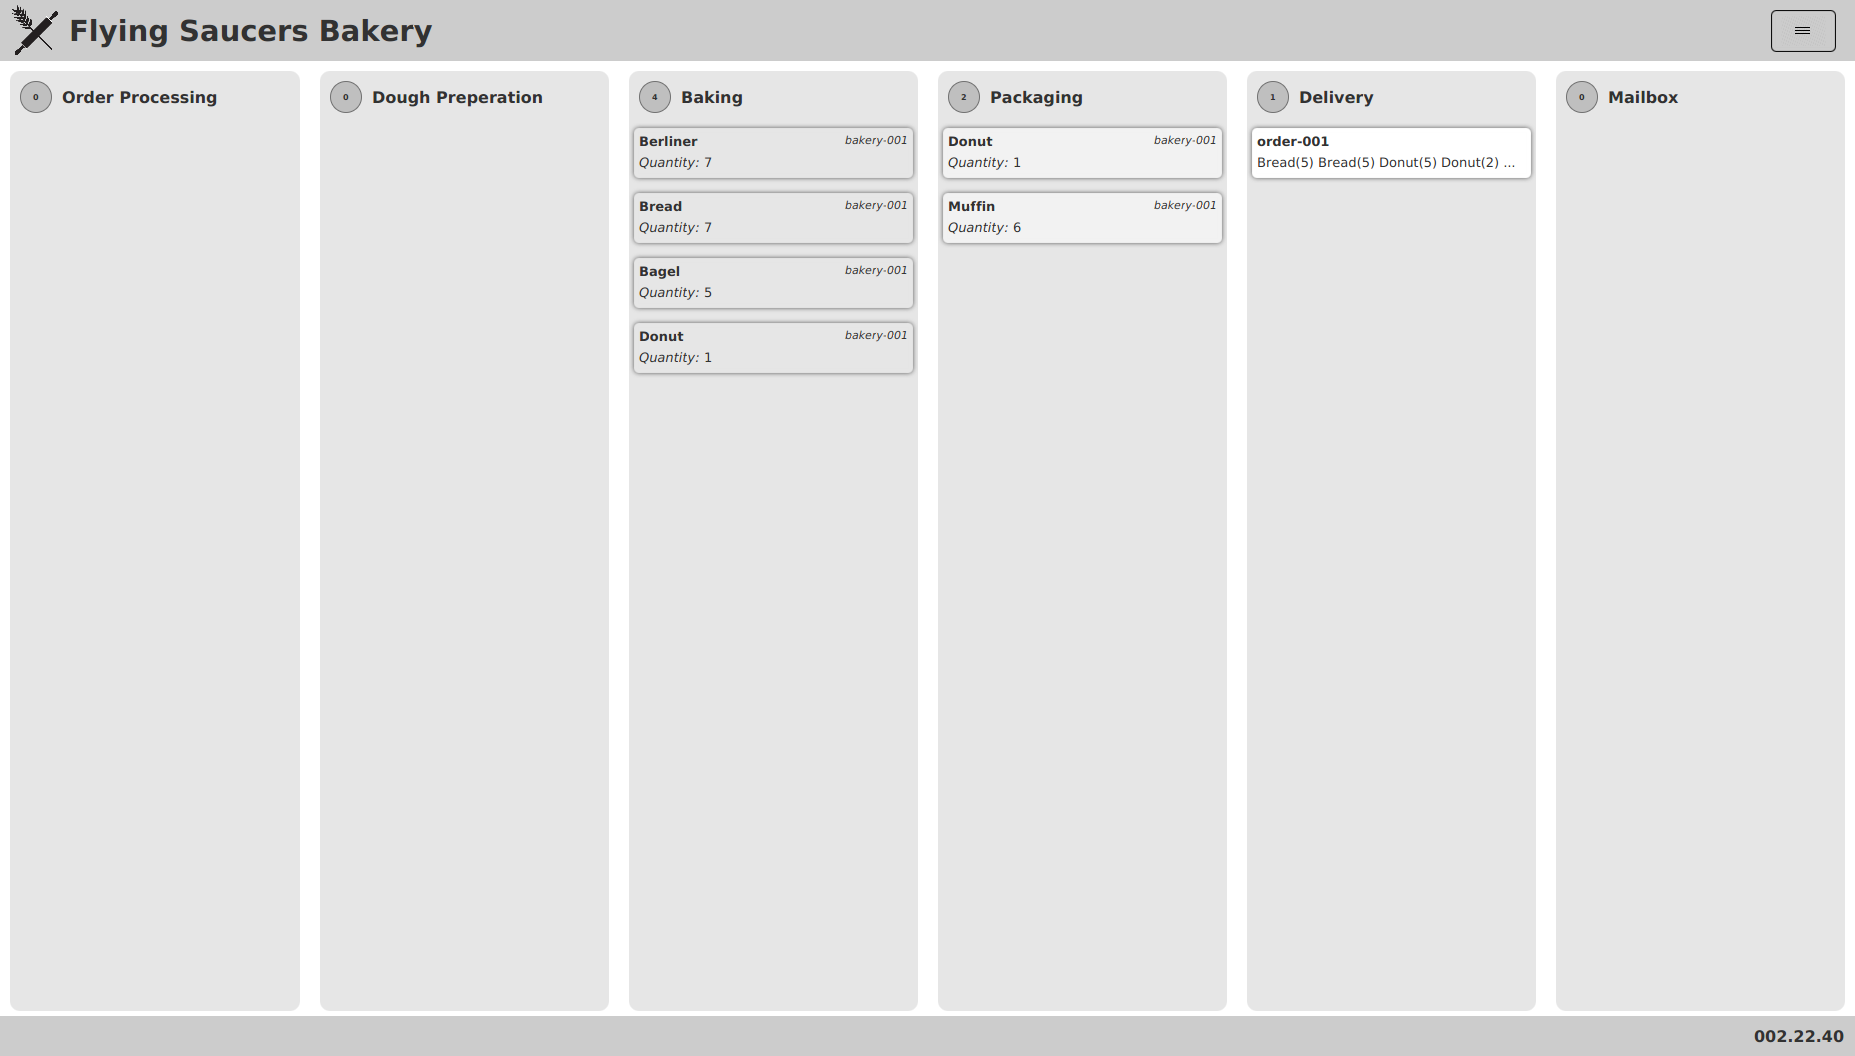
\includegraphics[width=0.99\linewidth]{visualizer-ui.png}
            \caption{Board visualization in progress}
        \end{figure}
\end{frame}

\begin{frame}
    \frametitle{\huge{Order Board Visualisation Agent}}
    \begin{figure}[H]
            \centering
            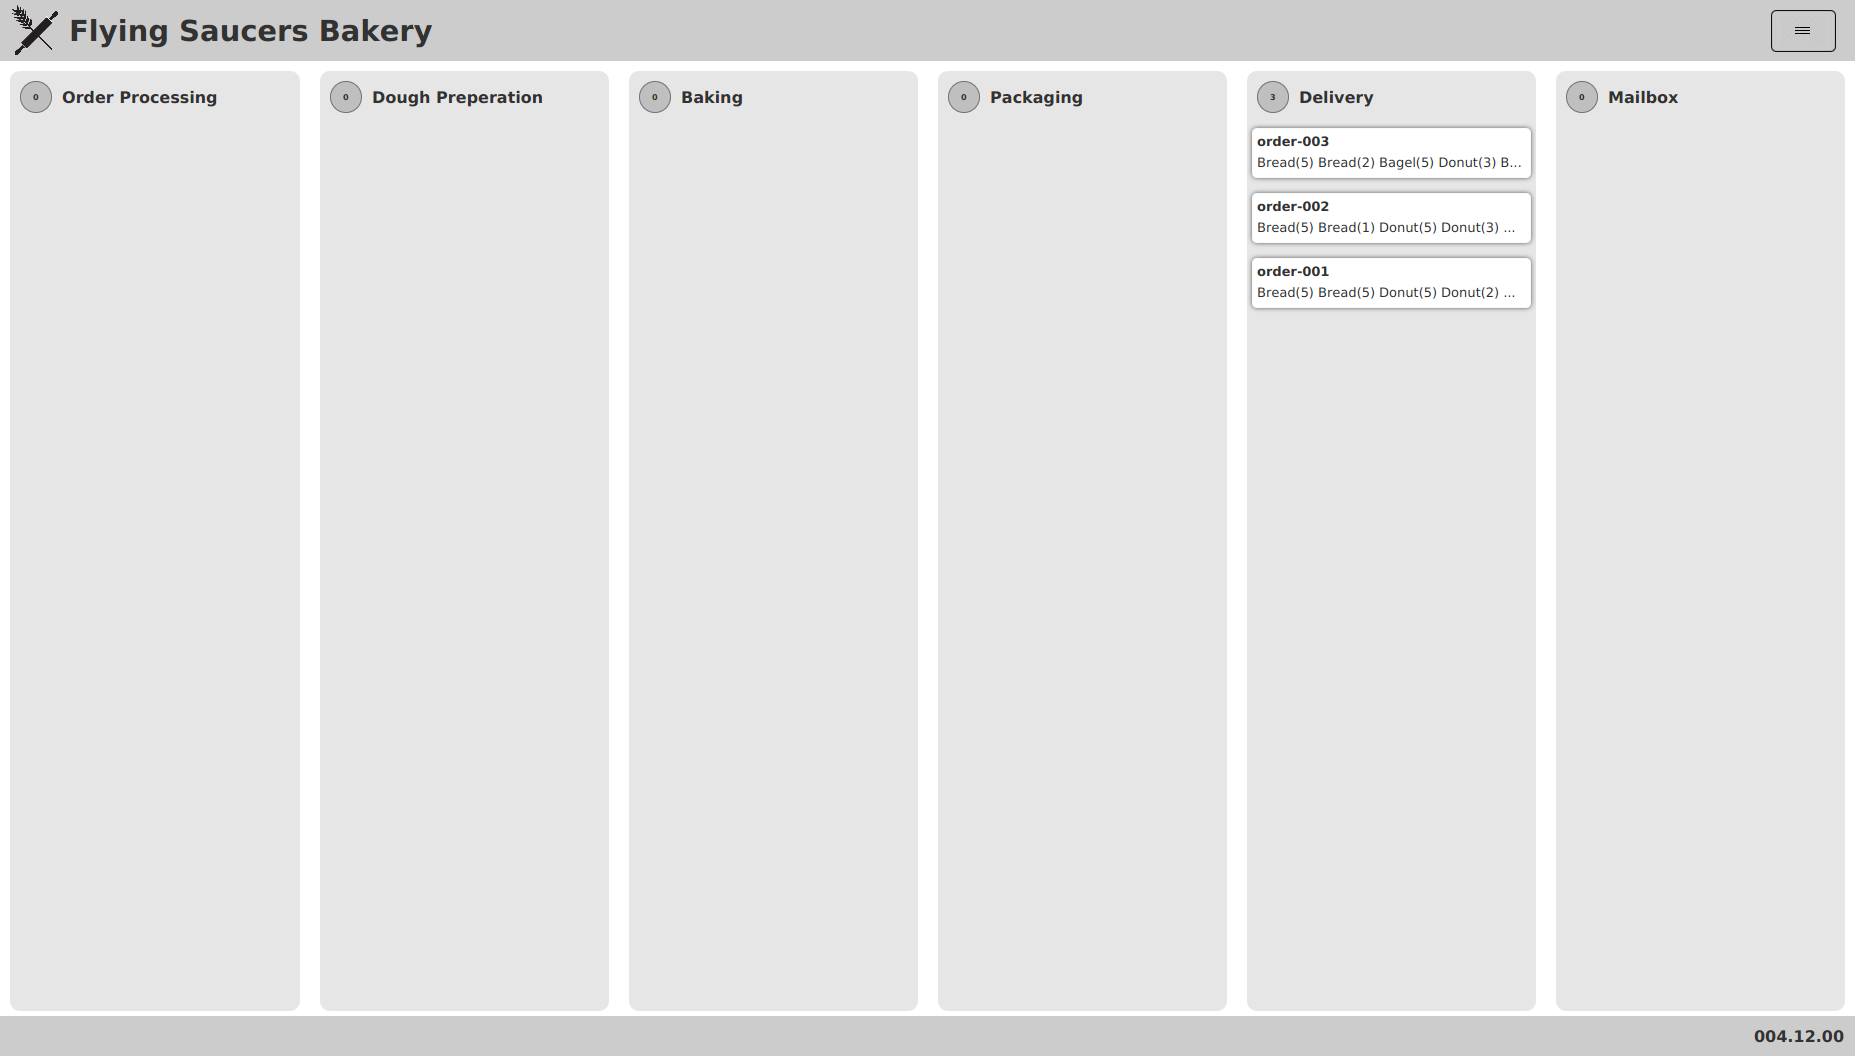
\includegraphics[width=0.99\linewidth]{visualizer-complete.png}
            \caption{Board visualization complete}
        \end{figure}
\end{frame}

\begin{frame}
    \frametitle{\huge{Order Board Visualisation Agent}}
    \begin{figure}[H]
            \centering
            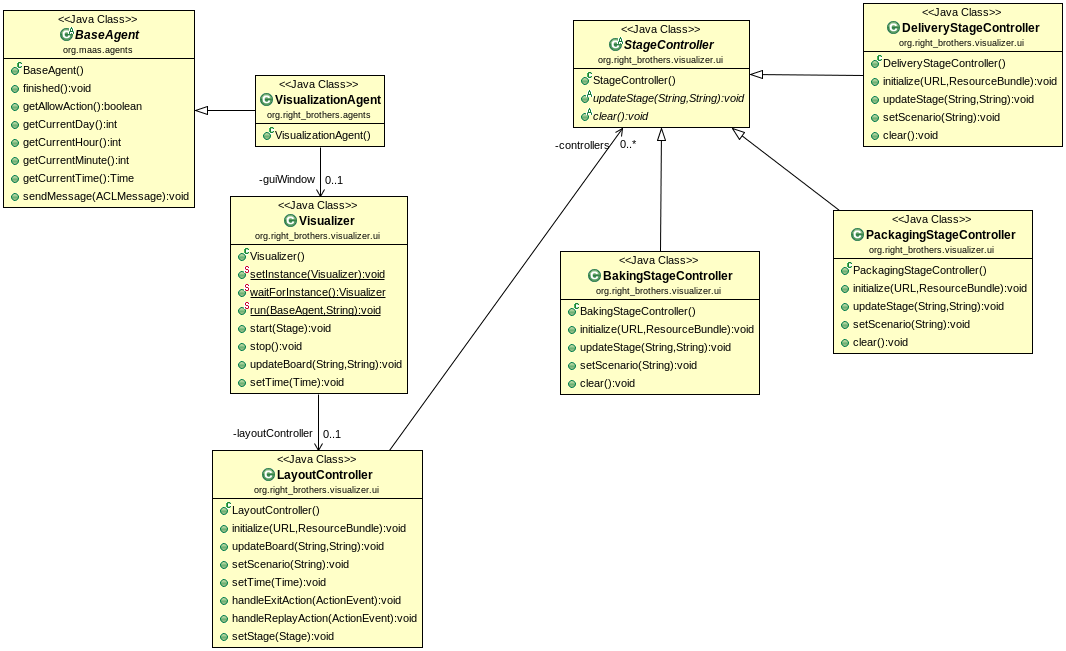
\includegraphics[width=0.99\linewidth]{class-diagram.png}
            \caption{Class diagram of the major classes of the visualizer}
        \end{figure}
\end{frame}

\begin{frame}
    \Huge{\centerline{Thank you}}
    \Huge{\centerline{Demo}}
\end{frame}


%\begin{frame}
%    \frametitle{\huge{Blocks of Highlighted Text}}
%    \begin{block}{Block 1}
%        Lorem ipsum dolor sit amet, consectetur adipiscing elit. Integer lectus nisl, ultricies in feugiat rutrum, porttitor sit amet augue. Aliquam ut tortor mauris. Sed volutpat ante purus, quis accumsan dolor.
%    \end{block}
%\end{frame}
%
%\begin{frame}
%    \frametitle{\huge{Multiple Columns}}
%    \begin{columns}[t]
%        \column{.45\textwidth}
%        \textbf{Heading}
%        \begin{enumerate}
%            \item Statement
%        \end{enumerate}
%        \column{.5\textwidth}
%        Lorem ipsum dolor sit amet, consectetur adipiscing elit. Integer lectus nisl, ultricies in feugiat rutrum, porttitor sit amet augue. Aliquam ut tortor mauris. Sed volutpat ante purus, quis accumsan dolor.
%    \end{columns}
%\end{frame}
%
%\begin{frame}
%    \frametitle{\huge{References}}
%        \footnotesize{
%        \begin{thebibliography}{1}
%            \bibitem[Smith, 2012]{p1} John Smith (2012) Some pub, some date
%        \end{thebibliography}
%}
%\end{frame}
%
%\begin{frame}
%    \Huge{\centerline{Thank you}}
%\end{frame}
\end{document} 
